\documentclass[twocolumn,times]{aastex62}

% these lines seem necessary for pdflatex to get the paper size right
\pdfpagewidth 8.5in
\pdfpageheight 11.0in

\usepackage[T1]{fontenc}
\usepackage{epsf,color,amsmath}

\usepackage{cancel}

\newcommand{\sfrac}[2]{\mathchoice%
  {\kern0em\raise.5ex\hbox{\the\scriptfont0 #1}\kern-.15em/
    \kern-.15em\lower.25ex\hbox{\the\scriptfont0 #2}}
  {\kern0em\raise.5ex\hbox{\the\scriptfont0 #1}\kern-.15em/
    \kern-.15em\lower.25ex\hbox{\the\scriptfont0 #2}}
  {\kern0em\raise.5ex\hbox{\the\scriptscriptfont0 #1}\kern-.2em/
    \kern-.15em\lower.25ex\hbox{\the\scriptscriptfont0 #2}} {#1\!/#2}}


\newcommand{\castro}{{\sf Castro}}
\newcommand{\maestro}{{\sf Maestro}}
\newcommand{\maestroex}{{\sf MAESTROeX}}

\newcommand{\nablab}{{\mathbf{\nabla}}}
\newcommand{\Ub}{\mathbf{U}}
\newcommand{\gb}{\mathbf{g}}
\newcommand{\omegadot}{\dot{\omega}}
\newcommand{\Sdot}{\dot{S}}
\newcommand{\ddx}[1]{{\frac{{\partial#1}}{\partial x}}}
\newcommand{\ddt}[1]{{\frac{{\partial#1}}{\partial t}}}
\newcommand{\odt}[1]{{\frac{{d#1}}{dt}}}
\newcommand{\divg}[1]{{\nablab \cdot \left (#1\right)}}

\newcommand{\Ic}{\mathcal{I}}
\newcommand{\smax}{{s_\mathrm{max}}}

\usepackage{bm}

\newcommand{\Uc}{{\bm{\mathcal{U}}}}
\newcommand{\Fb}{\mathbf{F}}
\newcommand{\Sc}{\mathbf{S}}

\newcommand{\xv}{{(x)}}
\newcommand{\yv}{{(y)}}
\newcommand{\zv}{{(z)}}

\newcommand{\ex}{{\bf e}_x}
\newcommand{\ey}{{\bf e}_y}
\newcommand{\ez}{{\bf e}_z}

\newcommand{\Ab}{{\bf A}}
\newcommand{\Sq}{{\bf S}_\qb}
\newcommand{\Sqhydro}{{\Sq^{\mathrm{hydro}}}}
\newcommand{\qb}{{\bf q}}

\newcommand{\Shydro}{{{\bf S}^{\mathrm{hydro}}}}
\newcommand{\Rb}{{\bf R}}
\newcommand{\Rq}{{\bf R}}
\newcommand{\Adv}[1]{{\left [\mathcal{A} \left(#1\right)\right]}}
\newcommand{\Advt}[1]{{\left [\mathcal{\tilde{A}} \left(#1\right)\right]}}
\newcommand{\Advs}[1]{{\mathcal{A} \left(#1\right)}}

\setlength{\marginparwidth}{0.75in}
\newcommand{\MarginPar}[1]{\marginpar{\vskip-\baselineskip\raggedright\tiny\sffamily\hrule\smallskip{\color{red}#1}\par\smallskip\hrule}}

\newcommand{\fab}{{\sf Fab}}
\newcommand{\multifab}{{\sf MultiFab}}

\received{XXX X, XXXX}
\revised{XXX X, XXXX}
\accepted{XXX X, XXXX}
%% Command to document which AAS Journal the manuscript was submitted to.
%% Adds "Submitted to " the arguement.
\submitjournal{ApJ}


\begin{document}
%======================================================================
% Title
%======================================================================
\title{CASTRO: A New Compressible Astrophysical Solver. IV. Performance Portability and GPUs}

\shorttitle{CASTRO Performance Portability and GPUs}
\shortauthors{}


\correspondingauthor{Michael Zingale}

\collaboration{the Castro Development Team}

\author[0000-0003-2103-312X]{Ann S. Almgren}
\affil{Center for Computational Sciences and Engineering, Lawrence Berkeley National Laboratory}

\author[0000-0002-3185-9809]{Maria Barrios Sazo}
\affil{Department of Physics and Astronomy, Stony Brook University}

\author{Kevin Gott}
\affil{National Energy Research Scientific Computing Center}

\author[0000-0002-1530-781X]{Alice Harpole}
\affil{Department of Physics and Astronomy, Stony Brook University}

\author[0000-0003-0439-4556]{Max P.~Katz}
\affil{NVIDIA Corporation}

\author[0000-0003-2300-5165]{Donald Willcox}
\affil{Center for Computational Sciences and Engineering, Lawrence Berkeley National Laboratory}

\author[0000-0001-8092-1974]{Weiqun Zhang}
\affil{Center for Computational Sciences and Engineering, Lawrence Berkeley National Laboratory}

\author[0000-0001-8401-030X]{Michael Zingale}
\affil{Department of Physics and Astronomy, Stony Brook University}
\email{michael.zingale@stonybrook.edu}




%======================================================================
% Abstract and Keywords
%======================================================================
\begin{abstract}
We describe a performance portable version of the \castro\ hydrodynamics
code that is able to achieve excellent scaling on both CPU and GPU-based
supercomputers.
\end{abstract}

\keywords{hydrodynamics---methods: numerical}

%======================================================================
% Introduction
%======================================================================
\section{Introduction}\label{Sec:Introduction}

Supercomputer architectures have evolved a lot over the past
decades~\citep{bell:2015}.  Shared memory vector machines with custom
processors dominated early, displaced in the early 1990s by
distributed memory, massively parallel architectures built upon
commodity CPUs where the message passing interface (MPI) became the
dominant library for achieving parallelism.  As core counts increased,
threading because increasingly important, and OpenMP became the
standard for threading in high-performance computing, with hybrid
MPI+OpenMP approaches to parallelism.  In the race to increase
performance while keeping electrical power consumption reasonable,
accelerators were increasingly turned to, include GPUs and many-core
chips like the Intel Phi series.  Throughout this evolution, the simulation codes we use in
astrophysics had to continue adapt to keep pace with the new computing paradigms, or they will
not be able to run on the next generation of supercomputers.  In
particular, GPUs are dominant now, so existing algorithms need to be
ported to run on GPUs, or new codes need to be written from scratch
targeting the new architecture.

There are a number of descriptions of GPU-enabled astrophysical hydro
codes, including
\citet{gamer,cholla,fargo3d,pekkila:2017,caplan:2018,racz:2018,liska:2018,goz:2018,wang:2010,Padioleau2019,Bryan2014,Kulikov2014,Bedorf2012,Schive2018,Potter2016} \MarginPar{todo:
  group by AMR/no-AMR, GPU exclusive, Kokkos \citep{CarterEdwards2014}, ...}

GPU-enabled integration has been explored by \citep{brock:2015}.\MarginPar{XNet paper?}


In this paper, we describe our approach to performance portability
with the \castro\ multiphysics simulation code.  We choose not to use
a framework like Kokkos but instead we implement the mechanism for
offloading compute kernels to GPUs inside of the AMReX adaptive mesh
refinement library itself.  Our goal is to have the same computational
kernels run efficiently on CPUs (including manycore processors) and
GPUs.  Early GPU results with a version of \castro\ were described in
\citet{astronum:2017}.  Here, we describe the work we needed to do to
enable this portability and show performance metrics for a reacting
flow problem in astrophysics.


\subsection{The Castro hydrodynamics code}

\castro\ development began with \cite{castro}, with the goal of
creating an astrophysical hydrodynamics code using a modern adaptive
mesh refinement library with space- and time-refinement (BoxLib at the
time) and unsplit hydrodynamics techniques.  \castro\ now uses the
AMReX adaptive mesh refinement library to handle the computational
grid, memory management, and parallelism, and the \castro\ and AMReX
developers work closely together to The initial application area was
nuclear astrophysics, including core-collapse supernovae, so it was
designed to work with a general equation of state~\citep{zingalekatz}
and arbitrary nuclear reaction networks, and with radiation transport
(through flux limited diffusion, \citealt{castro2,castro3}).  It
includes full self-gravity using multigrid methods with isolated
boundaries \citep{katz:2016}.  Finally, \castro\ also acted as the
compressible counterpart to our low Mach number hydrodynamics code
\maestro, sharing much of the same infrastructure, and allowing for
simulations to be restarted from the low Mach regime into the
compressible regime~\citep{malone:2014}.

\castro\ has been used for science investigations of various different
progenitor models of Type Ia
supernova~\citep{malone:2014,katz:2016,polin:2019}, exoplanet
dynamics~\citep{ryu:2018}, core-collapse and population III
supernovae~\citep{chen:2014,dolence:2015,chen:2017}, and X-ray
bursts~\citep{astronum:2018}.

\castro\ is developed using a fully open-development model, with the
code managed in git and hosted on
github\footnote{\url{https://github.com/amrex-astro/Castro/}}.
Contributions from the community are welcomed via github issues and
pull requests.  For the science projects that the core development
team are working on, all problem setup, input files, auxillary data,
and anything else needed for the science is stored in the main github
repo, allowing for the community to contribute to the science and
reproduce results as they are published.

\section{Performance portable compute kernels}

In \castro\ the domain is decomposed into a number of grids at various
levels of refinement.  A single grid and its associated data is called
a \fab, and its location in space is specified uniquely by the index
of its lower left cell, typically called {\tt lo}, and its upper right
cell, {\tt hi}, in a global index space for that level of refinement.
The collection of all the \fab s at a given level of refinement is
called a \multifab.  Time advancement proceeds by advancing all of the
grids at the coarsest level through a timestep $\Delta t$, and then
the grids at the next refinement level through {\tt rr} timesteps of
$\Delta t/\mathtt{rr}$, where {\tt rr} is the refinement ratio between
the levels, typically 2 or 4.  At that point, the two levels are at
the same time and a synchronization is done, as discussed in \cite{castro}.

\begin{figure*}[t]
\centering
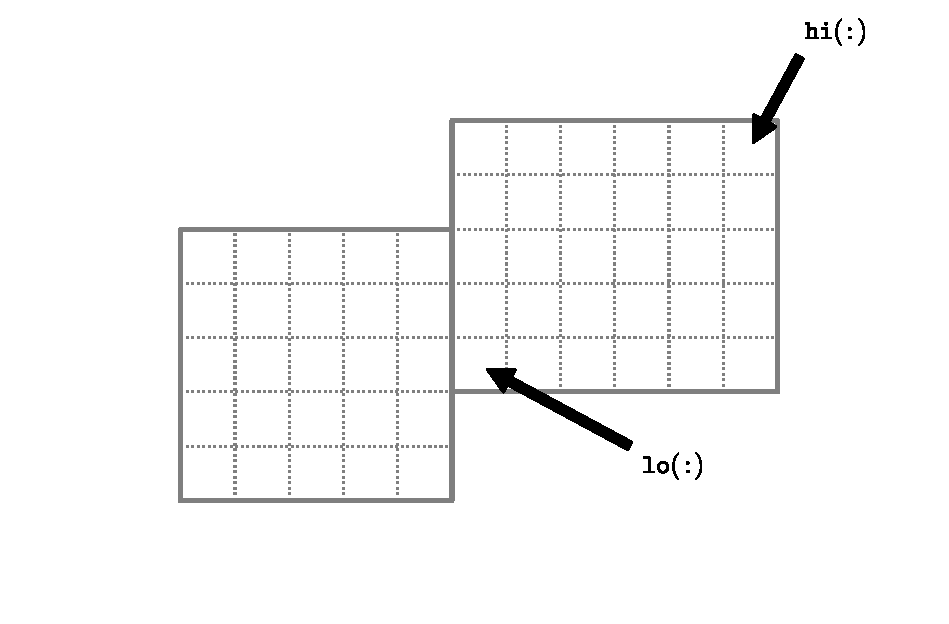
\includegraphics[width=0.33\textwidth]{gpu_1} 
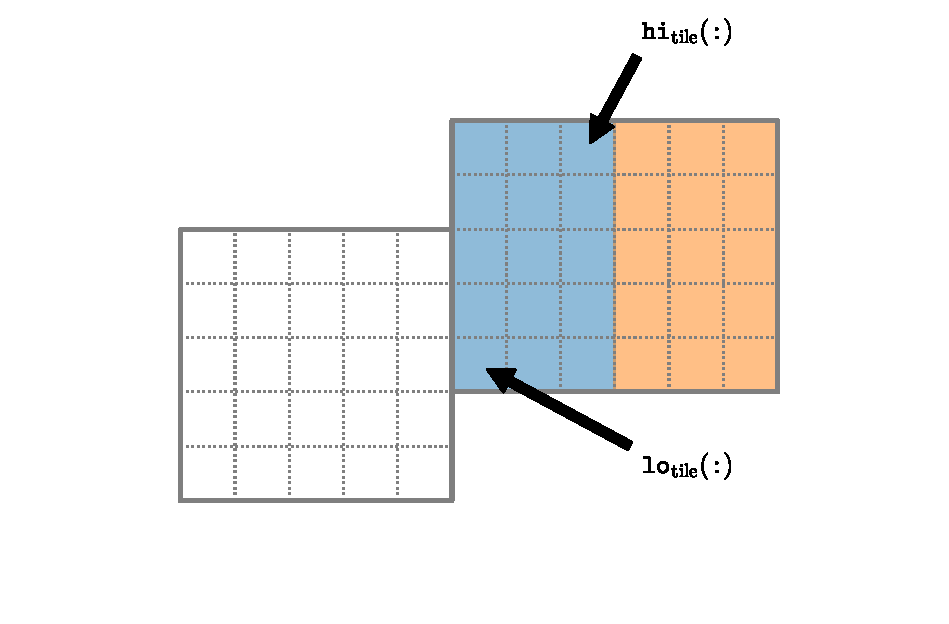
\includegraphics[width=0.33\textwidth]{gpu_2} 
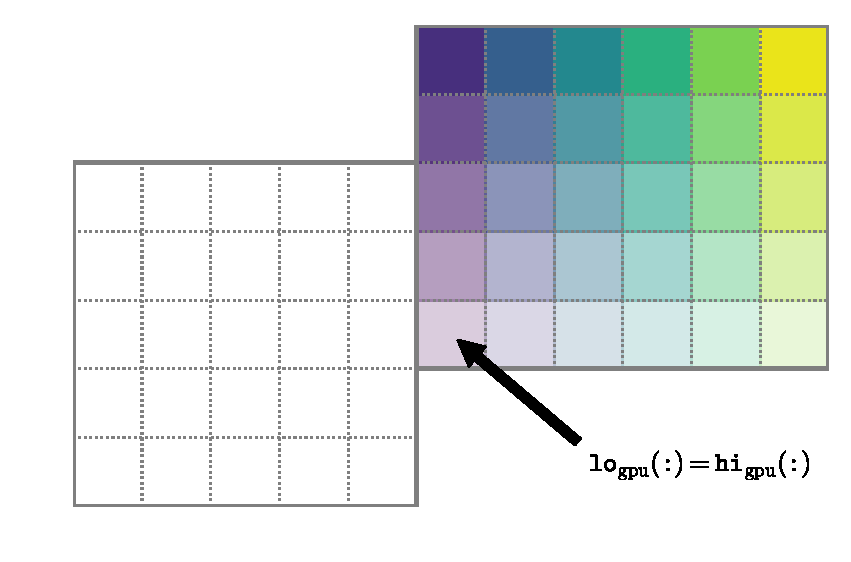
\includegraphics[width=0.33\textwidth]{gpu_3}
\caption{\label{fig:loops} Examples of distributing the work inside a
  grid patch.  On the left is the pure MPI approach.  An entire patch
  is assigned to a MPI task and the work loop runs over all of the
  cells in the grid, $\mathtt{lo:hi}$.  At the center is the
  tile-based MPI+OpenMP approach.  Again the grid is owned by an MPI
  task, but now it is logically subdivided into files (two shown
  here), and each tile is assigned to an OpenMP thread.  Each thread
  loops only over its tile, where the bounds are now given as
  $\mathtt{lo_{tile}:hi_{tile}}$.  Finally on the right is a GPU
  approach.  As with the others, the grid is owned by an MPI task but
  now each zone is assigned to a different GPU thread on the
  accelerator.  This is achieved by calling the same compute kernels,
  with $\mathtt{lo_{gpu}:hi_{gpu}}$ now corresponding to a single cell.}
\end{figure*}

The main drivers in Castro, including the memory management and
parallelism are written in C++.  The vast majority of the compute
kernels are written in modern Fortran, although with time we are
converting these to C++ as well.

\subsection{Offloading to GPUs}

GPUs achieve their performance by having a large number of threads
(1000s) that can execute the same instructions on multiple pieces of
data (a SIMD approach). \MarginPar{Max will not like this desciption.}
In modern supercomputers, like Summit at OLCF, more than 95\% of the
theoretical floating point performance is from the
GPUs \MarginPar{cite?}.  The main bottleneck with these hybrid systems
is copying the data back and forth between the main memory accessible
to the CPU and the memory on the GPU.  Therefore, to get the best
perfomance, we want to copy the data once onto the GPUs, operate as
much as possible on it while it is on the GPUs, and then copy back to
CPUs only when needed.  To simplify this data transfer, we use CUDA
managed memory.\MarginPar{more here}.  This approach will require us
to write all of our code in a manner that can be run on the GPUs.  We
discuss some of the issues here in this section.

There are several approaches to offloading a compute kernel to GPUs,
including the directive-based OpenACC and OpenMP, and the
NVIDIA-specific CUDA library.  For the present work, we use CUDA,
although our approach can mix the use of the directive-based
offloading instead of using pure CUDA.  This is something we will
explore in the future.  

CUDA Fortran is not as well supported as CUDA C/C++.  In particular,
CUDA Fortran does not automatically create both the host and device
kernel, necessitating one to do this themselves.  Usually this means
having two copies of a source routine, one marked up with device
attributes.  Keeping them in sync essentially requires that this
action be scripted, but in our experience, this scripting is fragile
because of the need to deal with Fortran syntax, preprocessor
directives, ...  Thus the pure CUDA route for the compute kernels
makes the most sense with C/C++ kernels, and not Fortran kernels.






\subsection{Example of advancing a grid}

Describe mfiter structure

Describe MPI, MPI+OpenMP w/ tiling, MPI + CUDA


\subsection{Summary of changes required}

The main hydrodynamics solver in \castro\ is an unsplit corner
transport upwind \citep{ppmunsplit} piecewise parabolic method
\citep{ppm} scheme.  This uses full corner coupling, requiring a
number of transverse Riemann problem solutions.


Boundary conditions require special attention---threadblock must include
all zones that participate in the boundary.

\section{Reaction networks}

The reaction update requires solving a system of ordinary differential
equations (ODEs).  Astrophysical reaction networks are notoriously
stiff, so implicit integrators are used (see,
e.g.\ \citealt{timmes:1999}).  \castro\ uses the VODE integrator
\citep{vode} which implements a variable order backward difference
implicit method to advance the system.  This requires the network to
provide a Jacobian as well as a routine to evaluate the righthand side
of the reaction ODE system.  It is these evaluations that dominate the
floating point work.  For integrating the system on GPUs, our approach
is to put the entire ODE integration on GPUs: the evaluation of the
righthand side and Jacobian as well as the driver which subcycles in
time to integrate the system to the desired tolerance.  VODE is
written in old Fortran, with numerous deprecated features that are not
supported in CUDA Fortran (like {\tt go to} statements and {\tt
  common} blocks).  We updated the code to eliminate these unsupported
statements, using more modern Fortran constructs.  The resulting
codebase is called VODE90 and serves as our GPU integrator.  \MarginPar{more here from Don}

\section{Performance}

On summit, we create a resource set with 1 MPI, 1 GPU, and 7 threads,
and there are 6 resource sets per node.

Do we also want to run on Cori?

Our current focus is on offloading the hydrodynamics and reactions to
GPUs, so we will achieve the best GPU performance for problems without
self-gravity.

\subsection{Pure hydrodynamics}

\subsection{Reaction test}

To understand the GPU performance of the reactions, we run a simple pure reaction test.  \MarginPar{is this {\tt test\_react}?}

\subsection{X-ray burst}

The {\tt flame\_wave} problem\footnote{Found in {\tt Castro/Exec/science/flame\_wave/}} in \castro\ was described in
\cite{astronum:2018}.  This problem explores the lateral propagation
of a helium deflagration across a neutron star in a plane-parallel
atmosphere.  The Castro PPM CTU hydrodynamics solver is used, with a
constant gravitational acceleration, and the problem is solved in the
corotating frame, where the Coriolis forces acts to balance the
lateral spreading in the atmosphere via geostrophic balance.  For the
microphysics, we use the general stellar equation of state of
\citep{timmes_swesty:2000} and the stellar conductivity described in
\citep{Timmes00}.  The science goal of the problem is to understand the
dynamics of a resolved burning front in X-ray bursts.  For this work,
this problem serves as an ideal reacting flow problem to benchmark
GPUs with.  All of the necessary physics: hydrodynamics, equation of
state, thermal conductivities, reactions, hydrodynamic source terms,
and thermal diffusion are run on the GPU.  We look at two different
reaction networks, a 7-isotope alpha network and a 13-isotope alpha
network~\citep{iso7}.



\section{Summary}

Self-gravity is the next important physics module that needs to be
developed for GPUs.  \castro\ uses either geometric multigrid,
implemented via AMReX, or a multipole expansion to solve for the
gravitational potential.  With Strang splitting of the reactions, it
is possible to asynchronously solve for the gravitational potential on
CPUs while solving the second-half of the reaction system on GPUs,
since the operator split approach does not change density via
reactions.  This is the approach we will explore in the near future
for self-gravitating reacting flows.

The Nyx cosmological code branched from \castro\ some time ago, but
they share a lot of the same compute kernels, so it should porting the
GPU-based hydro solver to Nyx is straightforward (and already in
progress).

We will also begin using the same ideas described here to port the
hydrodynamics and reactions in \maestroex\ to GPUs.  The projection of
the velocity field will remain on CPUs in the near future.


\software{MPICH, GCC, Castro, AMReX, python, matplotlib}

\facilities{OLCF, NERSC}

\acknowledgements \castro\ is available at
\url{http://github.com/AMReX-Astro/Castro}.  The work at Stony Brook
was supported by DOE/Office of Nuclear Physics grant DE-FG02-87ER40317
and NSF award AST-1211563.  An award of computer time was provided by
the Innovative and Novel Computational Impact on Theory and Experiment
(INCITE) program.  This research used resources of the Oak Ridge
Leadership Computing Facility at the Oak Ridge National Laboratory,
which is supported by the Office of Science of the U.S. Department of
Energy under Contract No.\ DE-AC05-00OR22725.  In particular, we thank
OLCF for early access to the Summitdev platform, where we could
develop and debug our GPU approach.  We also thank NVIDIA Corporation
for the donation of a Titan X Pascal and Titan V used in this
research.  The GPU development of \castro\ benefited greatly from
numerous GPU hackathons arranged by OLCF.




%======================================================================
% References
%======================================================================

\bibliographystyle{aasjournal}
\bibliography{ws}

\end{document}
